\documentclass[10pt]{article}

\usepackage{epsfig}
\usepackage{times}
\usepackage{amsmath}
\usepackage{amssymb}
\usepackage{fancyvrb}
\usepackage{fancyhdr}
\usepackage{graphicx}
\usepackage{color}
\usepackage[colorlinks=true,urlcolor=blue]{hyperref}
\usepackage[svgname]{xcolor}

\topmargin -0.3in
\oddsidemargin 0in
\evensidemargin 0in
\headheight 12pt
\headsep 12pt
\textheight 8.85in
\textwidth 6.5in
\parindent 0pt

\raggedbottom

\def\beqa#1\eeqa{\begin{eqnarray}#1\end{eqnarray}}
\newcommand{\R}{{\cal{R}}}
\newcommand{\N}{{\cal{N}}}
\newcommand{\C}{{\cal{C}}}
\newcommand{\D}{{\cal{D}}}
\renewcommand{\S}{{\cal{S}}}
\newcommand{\bx}{{\bf{x}}}
\newcommand{\by}{{\bf{y}}}
\newcommand{\bX}{{\bf{X}}}
\newcommand{\bt}{{\bf{t}}}
\newcommand{\bw}{{\bf{w}}}
\newcommand{\bm}{{\bf{m}}}
\newcommand{\bv}{{\bf{v}}}
\newcommand{\bS}{{\bf{S}}}
\newcommand{\bM}{{\bf{M}}}
\newcommand{\bphi}{{\boldsymbol{\phi}}}
\newcommand{\bPhi}{{\boldsymbol{\Phi}}}
\renewcommand{\d}{{\textrm{d}}}
\newcommand{\Figref}[1]{Fig.~\ref{#1}}
\newcommand{\Eqref}[1]{Eq.~\ref{#1}} % The '~' stops breaking and gives correct spacing
\newcommand{\Eqrefs}[2]{Eqs.~\ref{#1},~\ref{#2}}

\newcommand{\bh}{{\bf{h}}}
\newcommand{\ba}{{\bf{a}}}
\newcommand{\bb}{{\bf{b}}}
\newcommand{\Z}{{\cal{Z}}}
\newcommand{\bmu}{{\boldsymbol{\mu}}}
\newcommand{\bSigma}{{\boldsymbol{\Sigma}}}

\pagestyle{fancyplain}
\lhead{\fancyplain{}{Homework 2}}
\rhead{\fancyplain{}{10-707: Deep Learning}}
\cfoot{\thepage}

\title{\textsc{Homework 2}} % Title

\newcommand{\outDate}{Oct 9, 2017}
\newcommand{\dueDate}{Oct 23, 2017 11:59 pm}

\author{Nikhil Malik \\
nmalik1@andrew.cmu.edu}

\date{}
\begin{document}
\maketitle
\setcounter{page}{1}

%\pagestyle{myheadings}
%\setcounter{page}{1}

%\markboth{\hfil STA 4273H, Assignment 1}{
%          \hfil STA 4273H, Assignment 1}

%\vspace*{-32pt}


\section*{Problem 1 (10 pts)}

Loss Function
\beqa 
J = -log(y_m) \\
\frac{\partial J}{\partial{\by}} = [0,0...,-1/y_m,....0] \\
\eeqa
Softmax Normalization
\beqa 
y_m = exp(x_m)/(\sum_k exp(x_k)) \\
\frac{\partial y_i}{\partial{x_j}} = y_i*[(i==j) - y_j] \\
\eeqa
Softmax Weights: Where $d_2$ is the dimensionality of two post max pool feature maps
\beqa 
x_i = \beta_i + \sum_{l=1}^2 \sum_{e=1}^{d_2} \sum_{f=1}^{d_2} w_{efi}^l * v_{ef}^l \\
\frac{\partial x_i}{\partial{\beta_i}} = 1 \\
\frac{\partial x_i}{\partial{w_{efi}^l}} = v_{ef}^l \\
\frac{\partial x_i}{\partial{v_{ef}^l}} = w_{efi}^l \\
\eeqa
Maxpool Operation
\beqa 
v_{ef}^l = max((a_{e*p+c,f*p+d}^l)_{d=0}^{p-1})_{c=0}^{p-1} \\
\eeqa
\begin{equation}
  \frac{\partial v_{ef}^l}{\partial{a_{gh}^l}}=\begin{cases}
    1, & \text{$a_{gh}^l$ was the max in max pool window }.\\
    0, & \text{otherwise}.
  \end{cases}
\end{equation}
\beqa 
\eeqa
Convolution Operation
\beqa 
a_{gh}^l = \theta_l + \sum_{u=0}^{k-1} \sum_{v=0}^{k-1} \theta_{uv}^l * input_{g*s + u, h*s + v} \\
\frac{\partial a_{gh}^l}{\partial{\theta_{ab}^l}} = \sum_{g,h} input_{g*s + a,h*s+b} \\
\eeqa
Chain rule expressions, where all the individuals components have been calculated above
\beqa 
\frac{\partial J}{\partial{\beta_i}} = \frac{\partial J}{\partial{\by}} * \sum_j (\frac{\partial y_j}{\partial x_i} * \frac{\partial x_i}{\partial{\beta_i}} ) \\
\frac{\partial J}{\partial w_{efi}^l} = \frac{\partial J}{\partial{\by}} * \sum_j (\frac{\partial y_j}{\partial x_i} * \frac{\partial x_i}{\partial{w_{efi}^l}} ) \\
\frac{\partial J}{\partial{\theta_{ab}^l}} = \frac{\partial J}{\partial{\by}} * \sum_j (\frac{\partial y_j}{\partial x_i} * \frac{\partial x_i}{\partial v_{ef}^l} * \sum_{e,f} ( \frac{\partial v_{ef}^l}{\partial{a_{gh}^l}} * \sum_{g,h} \frac{\partial  a_{gh}^l}{\partial{\theta_{ab}^l}} ) )
\eeqa

\section*{Problem 2 (10 pts)}

\beqa p(\bx) = \prod_{k=1}^K p(x_k | \textrm{pa}_k) \eeqa
We need to prove
\beqa \sum_{x_1,x_2,..x_K} p(\bx) = 1 \eeqa
\beqa \sum_{x_1,x_2,..x_K} p(\bx) = \sum_{x_1,x_2,..x_K} \prod_{k=1}^K p(x_k | \textrm{pa}_k) \eeqa
\beqa \sum_{x_1,x_2,..x_K} p(\bx) = \sum_{x_1,x_2,..x_K} p(x_K | \textrm{pa}_K)*\prod_{k=1}^{K-1} p(x_k | \textrm{pa}_k) \eeqa
\beqa \sum_{x_1,x_2,..x_K} p(\bx) = \sum_{x_1,x_2,..x_{K-1}} ( \sum_{x_K} p(x_K | \textrm{pa}_K))*\prod_{k=1}^{K-1} p(x_k | \textrm{pa}_k) \eeqa
\beqa \sum_{x_1,x_2,..x_K} p(\bx) = \sum_{x_1,x_2,..x_{K-1}} (1)*\prod_{k=1}^{K-1} p(x_k | \textrm{pa}_k) \eeqa
Repeating the same steps as above K-1 times.
\beqa \sum_{x_1,x_2,..x_K} p(\bx) = (1)*(1)* .. * (1) \eeqa
\beqa \sum_{x_1,x_2,..x_K} p(\bx) = 1\eeqa
This proves that the original representation was correctly normalized.


\section*{Problem 3 (10pts)}
\beqa
 E(\bv, \bh; \theta ) =
 -\sum_{i=1}^D \sum_{j=1}^P W_{ij} v_i h_j - \sum_{i=1}^D v_i b_i -
 \sum_{j=1}^P h_j a_j.
\eeqa

\beqa
 P_{\theta} (\bv,\bh) = \frac{1}{\Z} \exp(-E (\bv, \bh; \theta )) \\
\Z = \sum_{\bv, \bh} \exp(-E (\bv, \bh; \theta ))
\eeqa
Since $ h_2, h_3,...,h_P $ are not part of markov blanket of $h_1$, we can write
\beqa
 P_{\theta}(h_1,h_2...,h_P | \bv) = P_{\theta}(h_1 | \bv) * P_{\theta} (h_2...,h_P | \bv)
 \eeqa
Repeating the same step P times
\beqa
 P_{\theta}(h_1,h_2...,h_P | \bv) = P_{\theta}(h_1 | \bv) * P_{\theta}(h_2 | \bv) * ... * P_{\theta}(h_P | \bv) \\
  P_{\theta}(h_1,h_2...,h_P | \bv) = \prod_j P_{\theta}(h_j | \bv) \\
P_{\theta}(h_j | \bv) = \frac{1}{\Z_j} \exp(-E (\bv, h_j; \theta )) \\
P_{\theta}(h_j | \bv) = \frac{1}{\Z_j} \exp(\sum_{i=1}^D W_{ij} v_i h_j + \sum_{i=1}^D v_i b_i + h_j a_j) \\
P_{\theta}(h_j = 1 | \bv) = \frac{1}{\Z_j} \exp(\sum_{i=1}^D W_{ij} v_i + \sum_{i=1}^D v_i b_i +
 a_j) \\
P_{\theta}(h_j = 0 | \bv) = \frac{1}{\Z_j} \exp( \sum_{i=1}^D v_i b_i) \\
P_{\theta}(h_j = 1 | \bv) = P_{\theta}(h_j = 1 | \bv)/(P_{\theta}(h_j = 1 | \bv) + P_{\theta}(h_j = 0 | \bv)) \\
P_{\theta}(h_j = 1 | \bv) = \exp(\sum_{i=1}^D W_{ij} v_i + \sum_{i=1}^D v_i b_i +
 a_j)/(\exp(\sum_{i=1}^D W_{ij} v_i + \sum_{i=1}^D v_i b_i + a_j) + \exp(\sum_{i=1}^D v_i b_i)) \\
 P_{\theta}(h_j = 1 | \bv) = \exp(\sum_{i=1}^D W_{ij} v_i + a_j)/(\exp(\sum_{i=1}^D W_{ij} v_i + a_j) + 1) \\
 P_{\theta}(h_j = 1 | \bv) = 1/(1 + \exp(-\sum_{i=1}^D W_{ij} v_i - a_j)) \\
  P_{\theta}(h_j = 1 | \bv) = Sigm(\sum_{i=1}^D W_{ij} v_i + a_j)) \\
 \eeqa

This proves the original expression

\section*{Problem 4 (10 pts)}
\beqa
E(\bx,\by) = h \sum_i x_i - \beta \sum_{i,j} x_i x_j - \eta \sum_i x_i y_i,
\eeqa
\beqa
p(\bx,\by) = \frac{1}{\Z} \exp{(-E(\bx,\by)}
\eeqa

\begin{itemize}
\item (5 pts)

\beqa
E(x_1, ... x_k = 1, .. x_K,\by) = h \sum_{i{\neq}k} x_i - \beta \sum_{i{\neq}k,j} x_i x_j - \eta \sum_{i{\neq}k} x_i y_i + h -\beta \sum_{j{\in}ne({x_k})} x_j - \eta y_k
\eeqa
\beqa
E(x_1, ... x_k = -1, .. x_K,\by) = h \sum_{i{\neq}k} x_i - \beta \sum_{i{\neq}k,j} x_i x_j - \eta \sum_{i{\neq}k} x_i y_i - h +\beta \sum_{j{\in}ne({x_k})} x_j + \eta y_k
\eeqa

\beqa
E(x_1, ... x_k = 1, .. x_K,\by) - E(x_1, ... x_k = -1, .. x_K,\by) =  2h -2\beta \sum_{j{\in}ne({x_k})} x_j - 2\eta y_k
\eeqa

As per this expression the difference in energy depends only on neighbourhood of particular element of x.



\item (5 pts)

Substituting $\beta$ and h in expression above
\beqa
E(x_1, ... x_k = 1, .. x_K,\by) - E(x_1, ... x_k = -1, .. x_K,\by) =  -2\eta y_k
\eeqa

Given $\eta >= 0$ \\
If ${y_k} = 1$
\beqa
E(x_1, ... x_k = 1, .. x_K,\by) - E(x_1, ... x_k = -1, .. x_K,\by) = -2\eta \\
E(x_1, ... x_k = 1, .. x_K,\by) - E(x_1, ... x_k = -1, .. x_K,\by) < 0 \\
E(x_1, ... x_k = 1, .. x_K,\by) < E(x_1, ... x_k = -1, .. x_K,\by) \\
\eeqa
Lower value of energy corresponds to higher likelihood. Therefore ${x_k} = 1$

Similarly, if ${y_k} = -1$
\beqa
E(x_1, ... x_k = 1, .. x_K,\by) - E(x_1, ... x_k = -1, .. x_K,\by) = 2\eta \\
E(x_1, ... x_k = 1, .. x_K,\by) - E(x_1, ... x_k = -1, .. x_K,\by) > 0 \\
E(x_1, ... x_k = 1, .. x_K,\by) > E(x_1, ... x_k = -1, .. x_K,\by) \\
\eeqa
Hihger value of energy corresponds to lower likelihood. Therefore ${x_k} = -1$

From the two results above the most probable configuration of latent variables corresponds to ${y_k} = {x_k} $

\end{itemize}

\section*{Problem 5 (60 pts)}
\subsubsection*{Contrastive Divergence (CD), Autoencoders}


\subsubsection*{a) Basic generalization [20 points]}

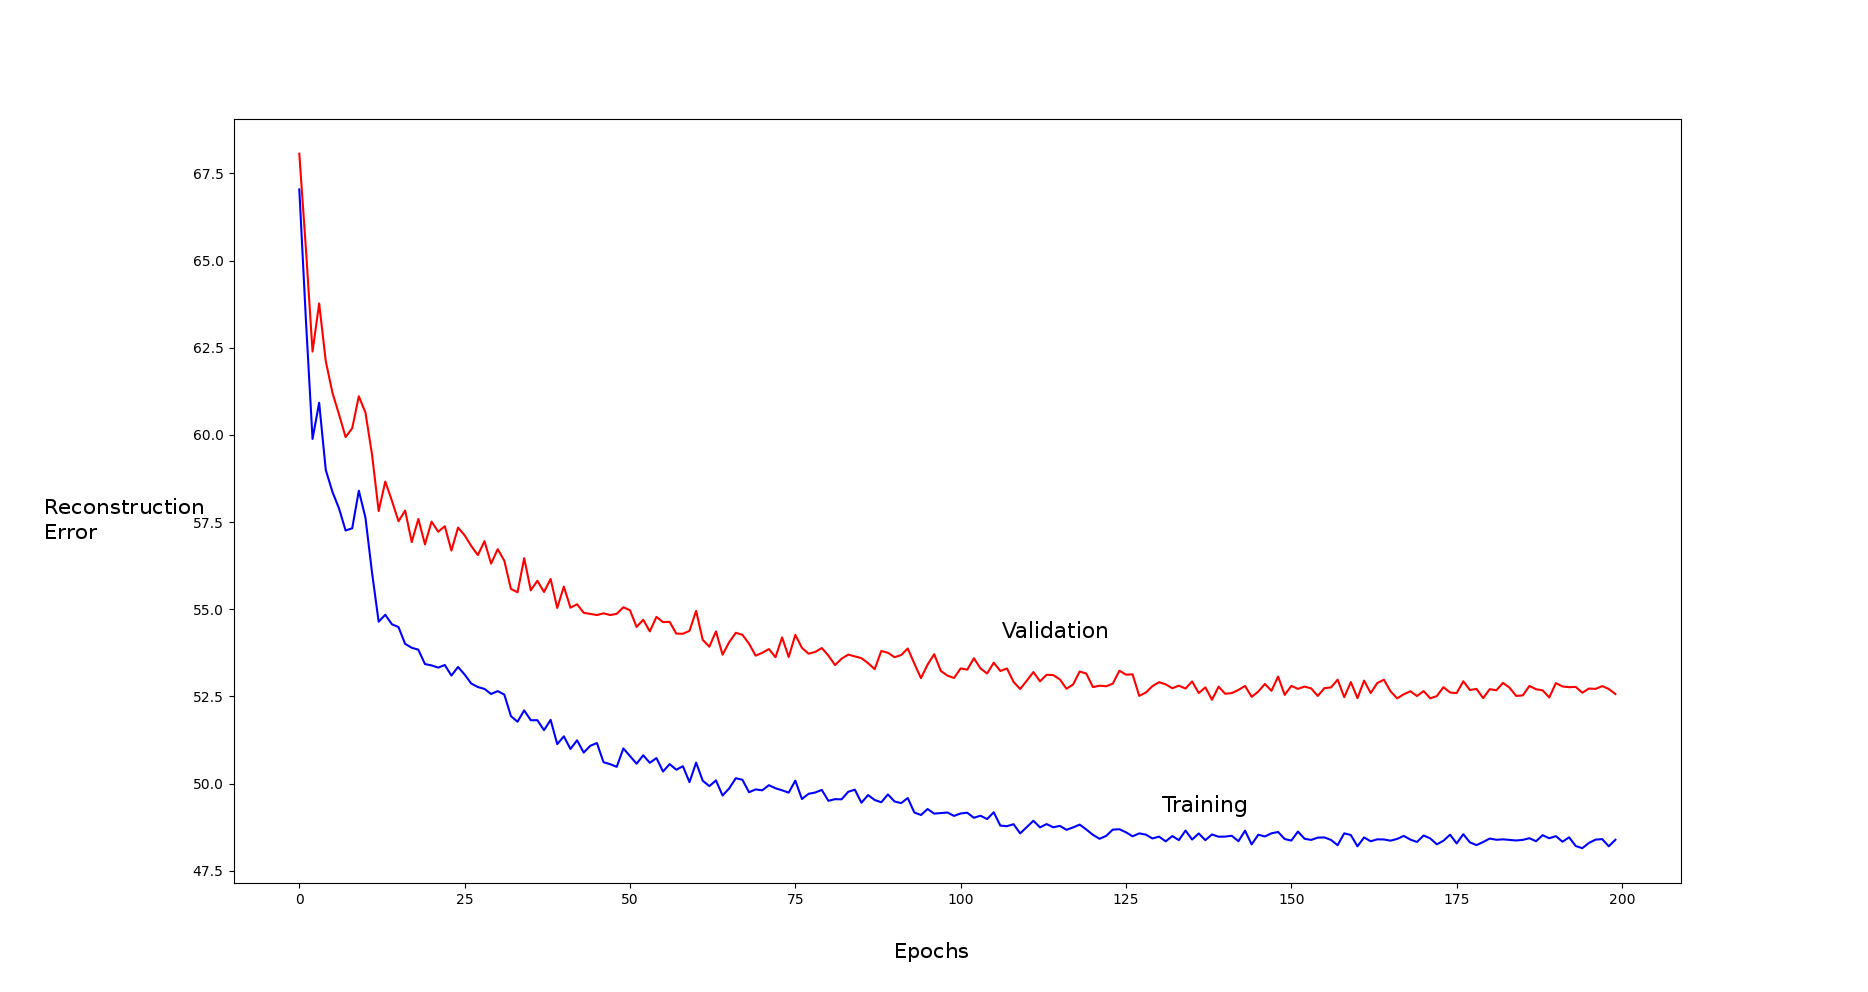
\includegraphics[scale=0.2]{rbm_recon_error.png}

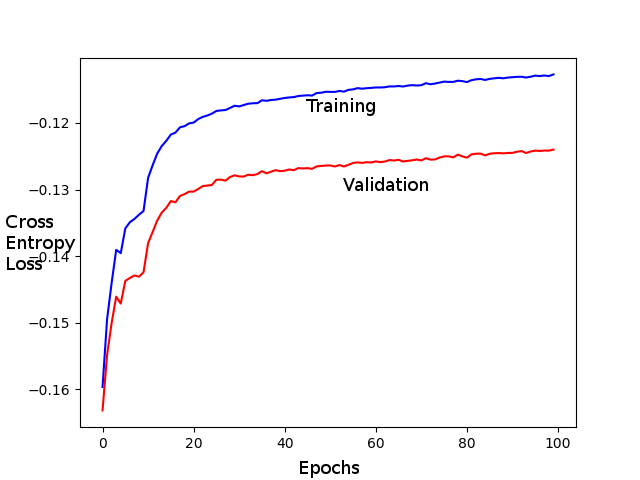
\includegraphics[scale=0.6]{rbm_loss.png}

Training set error goes down faster compared to validation set as expected. After 125 epochs the validation error stops reducing representing the generalization error region.

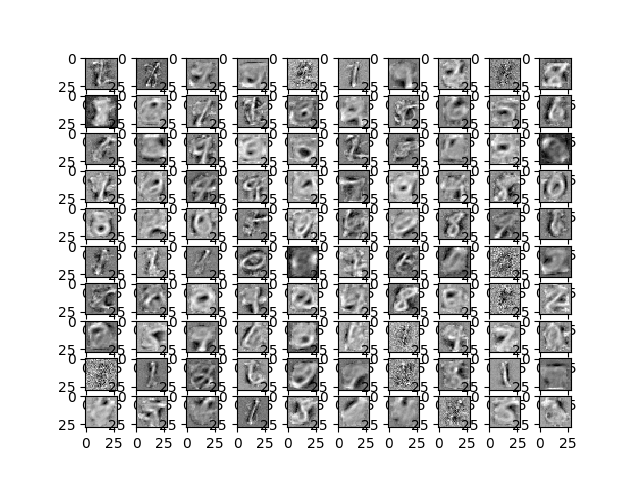
\includegraphics[scale=0.7]{rbm_weights.png}

The visualized Weights W do represent structure similar to original digits or components such as curves that look similar to components of the original digits.

\subsubsection*{b) Number of CD steps [5 points]}

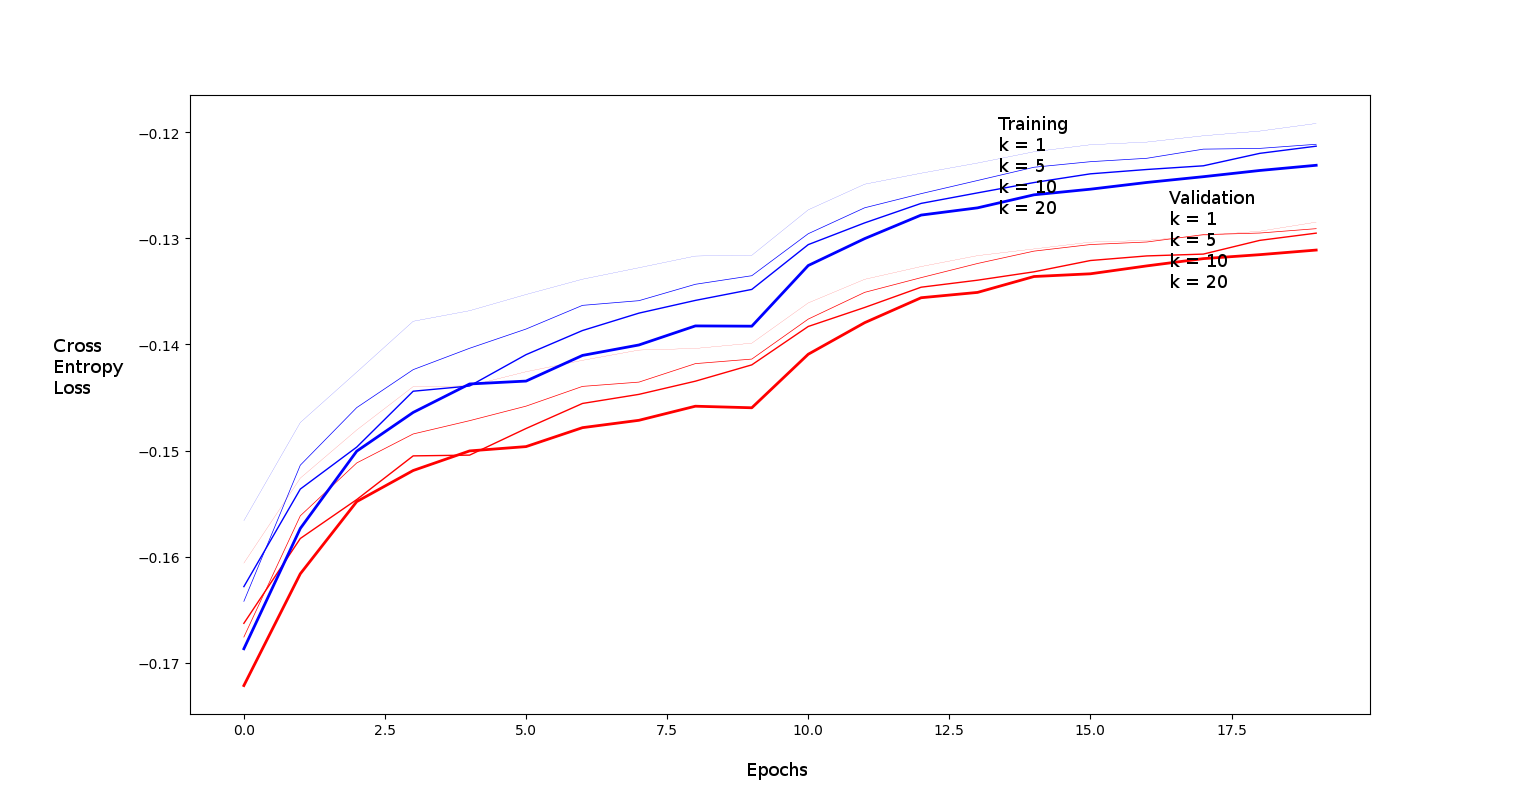
\includegraphics[scale=0.4]{rbm_k_experiment.png}

In terms of convergence of training accuracy, higher value of k (indicated by thicker lines in the figure) converges slowly compared to smaller values (indicated by thicker lines in the figure) i.e. k=1 converges the fastest.

However in terms of generalization error, k = 5 does the best. k = 10 is comparable to k = 5. While k = 1 has the highest generalization error. k = 20 underfits, at least untill 50 epochs compared to smaller values of k.
Discribe Observation

\subsubsection*{c) Sampling from the RBM model [5 points]}

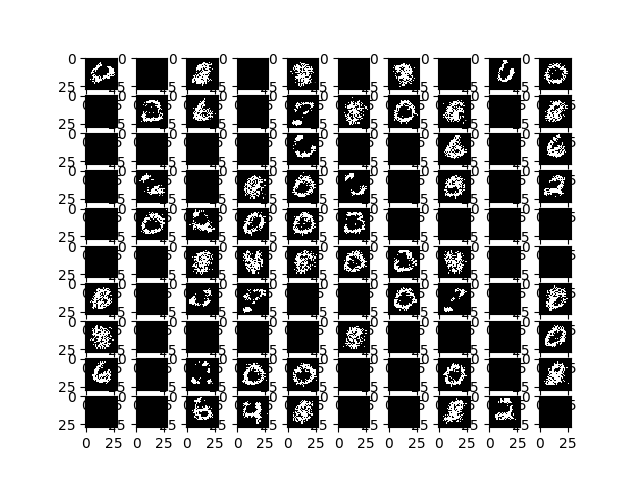
\includegraphics[scale=0.7]{digit_generation.png}

They do show a very rough structure of handwritten digits.

\subsubsection*{d) Unsupervised Learning as pretraining [5 points]}
  
\begin{figure}
  \caption{Figure A: Comparing Generalization for different initialization strategies}
  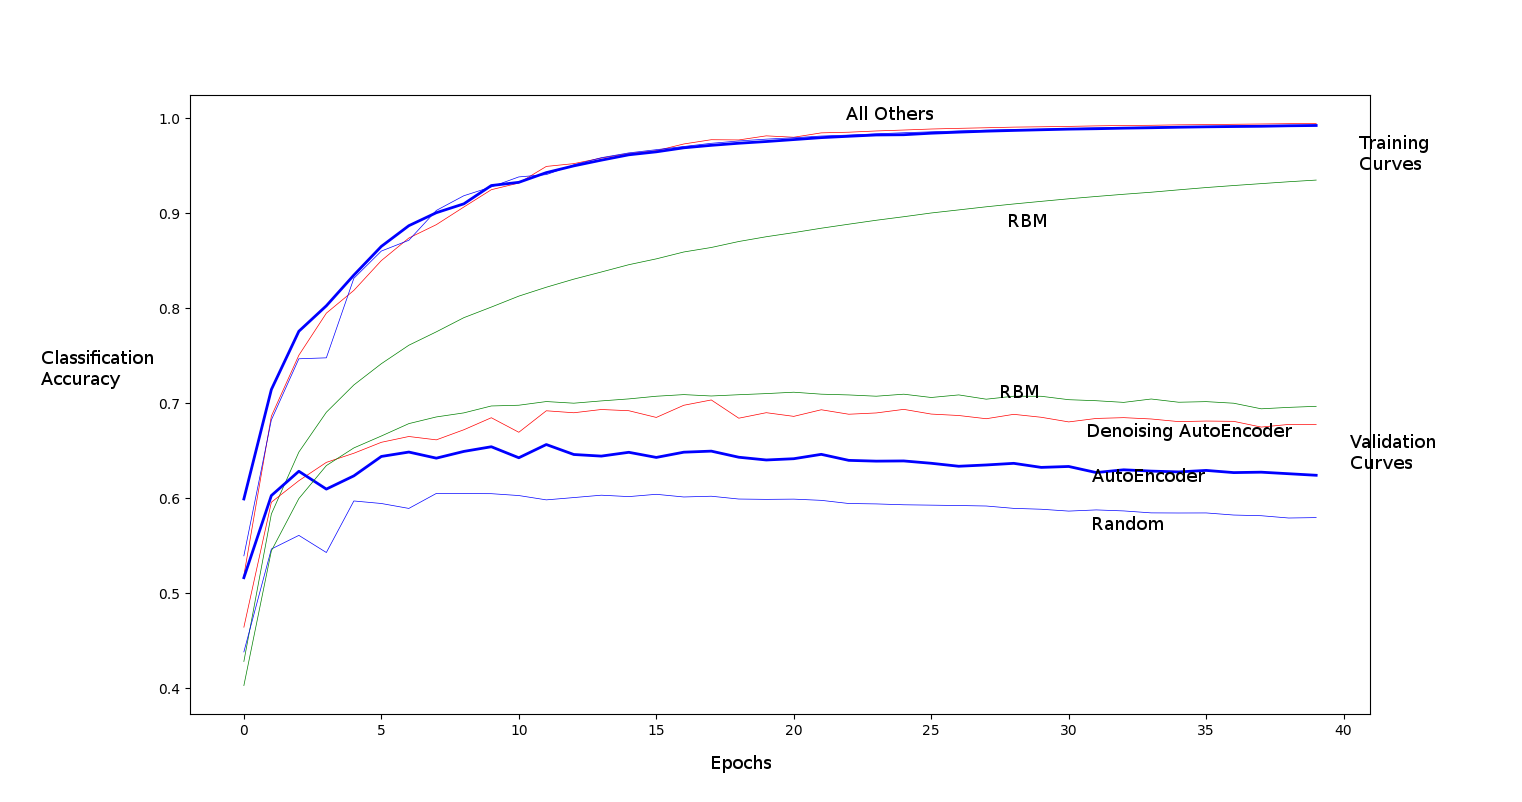
\includegraphics[scale=0.5]{classification_initialization_experiment_v1.png}
\end{figure}

Yes, rbm initialization imporves the model generalizability. It acheives the best validation accuracy, and tends to not over fit unlike all other initialization methods. (see Figure A)

\subsubsection*{e) Autoencoder [5 points]}

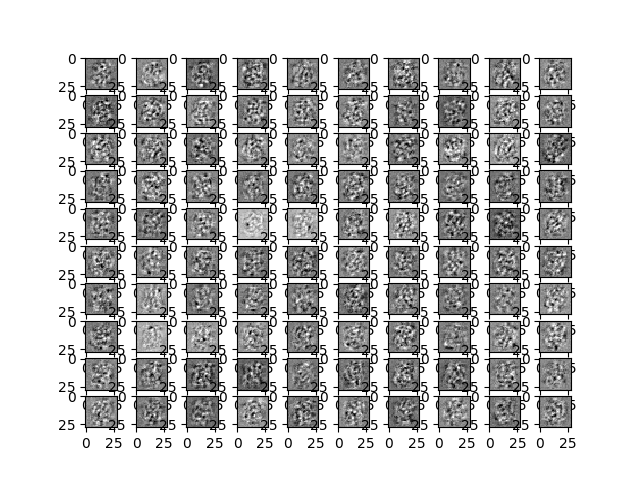
\includegraphics[scale=0.6]{ae_weights.png}
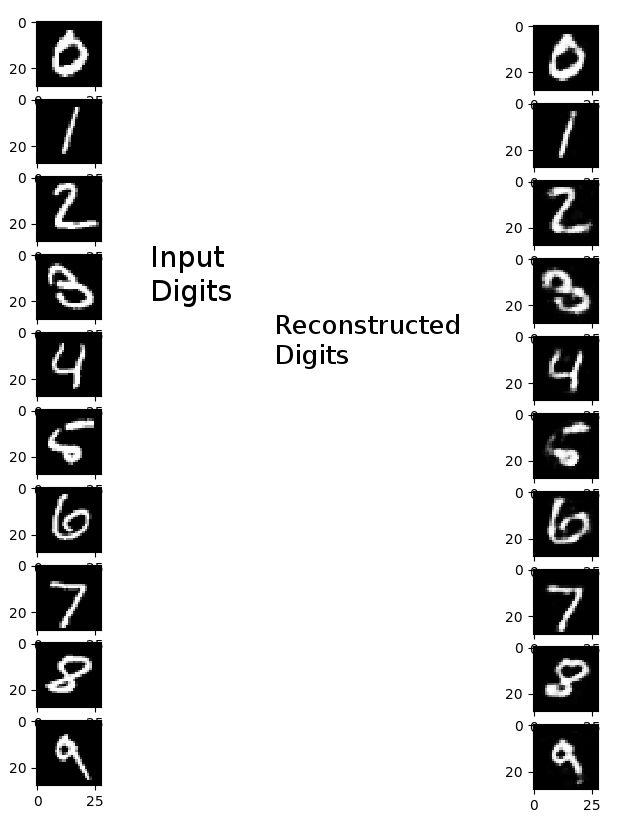
\includegraphics[scale=0.3]{ae_recon.png}

Unlike rbm, there is very limited structure to discern in the visualization of Auto encoder weights. Even so, the auto encoder is able to accomplish a fairly good reconstruction of the input digit.


The standard autoencoder does better than random initialization in terms of validation accuracy. However it still starts to overfit after 10 epochs or so. It doesn't offer the same generalizability as the rbm initialization. (see Figure A)
 

\subsubsection*{f) Denoising Autoencoder [10 points]}

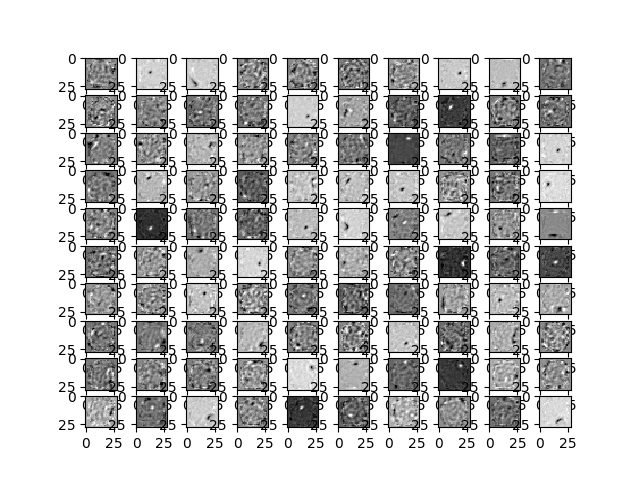
\includegraphics[scale=0.7]{ae_dropout_weights.png}
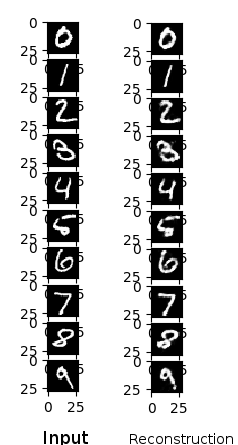
\includegraphics[scale=0.7]{ae_dropout_recon.png}

Compared to no drop out auto encoder, there is greater structure visible in the weight visualization. The reconstructed digits are also sharper compared to the standard autoencoder. The filters are still not as crisp as the rbm case.

\begin{figure}
  \caption{Figure A (repeated): Comparing Generalization for different initialization strategies}
  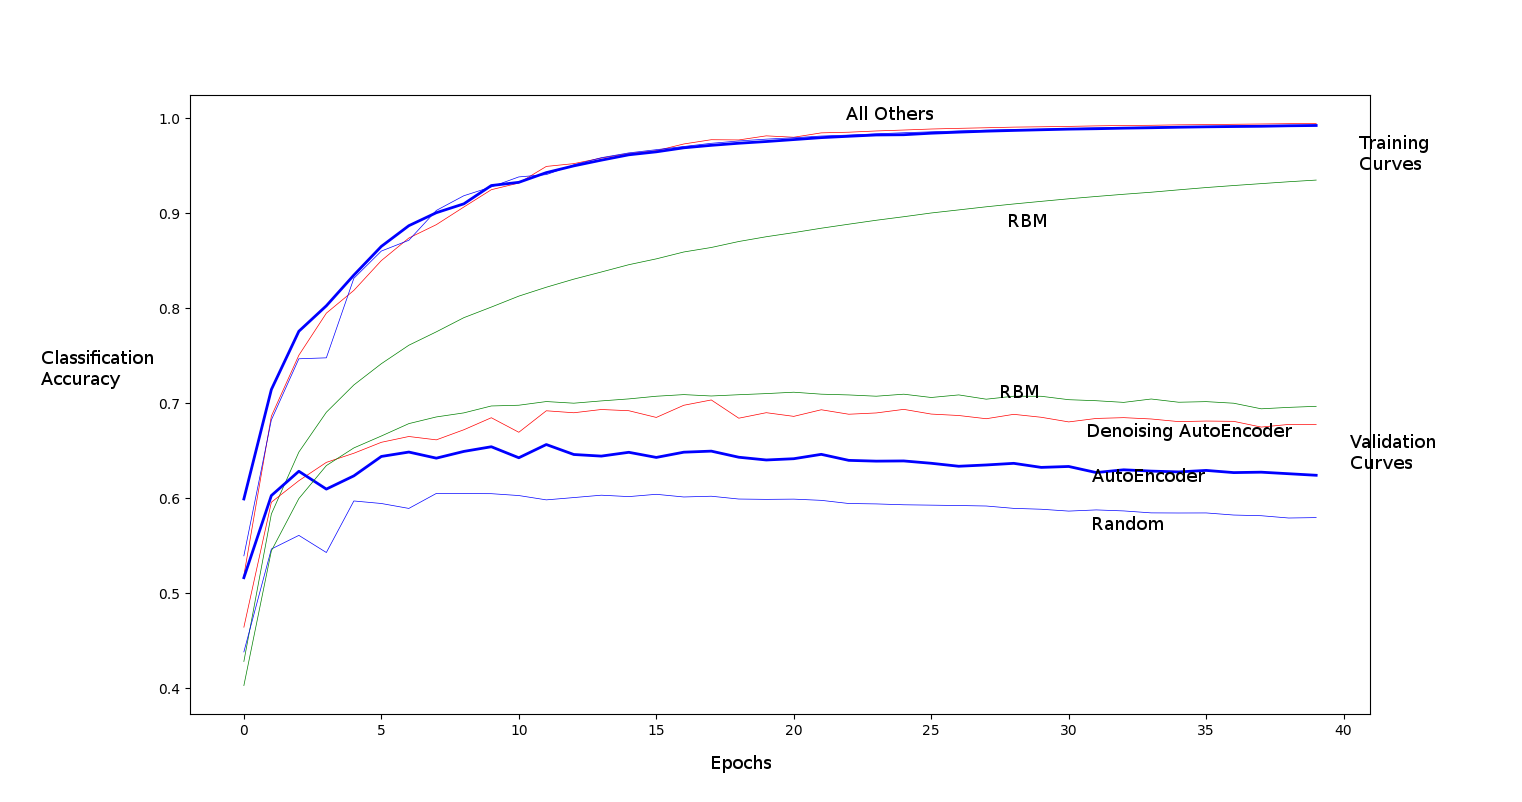
\includegraphics[scale=0.4]{classification_initialization_experiment_v1.png}
\end{figure}

The denoising autoencoder pre-training is an improvement over both random initialization and standard auto encoder. Compared to rbm initializations it performs as good or slightly worse on multiple attempts in terms of validation accuracy and generalizability. (see Figure A)


\subsubsection*{g) Number of hidden units [10 points]}

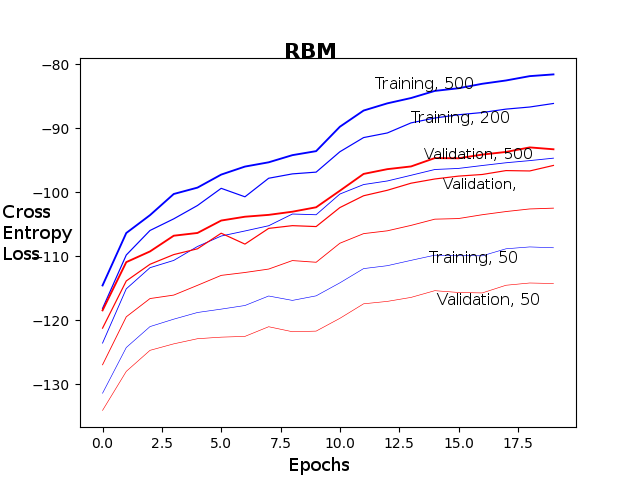
\includegraphics[scale=0.6]{rbm_hu_experiment.png}

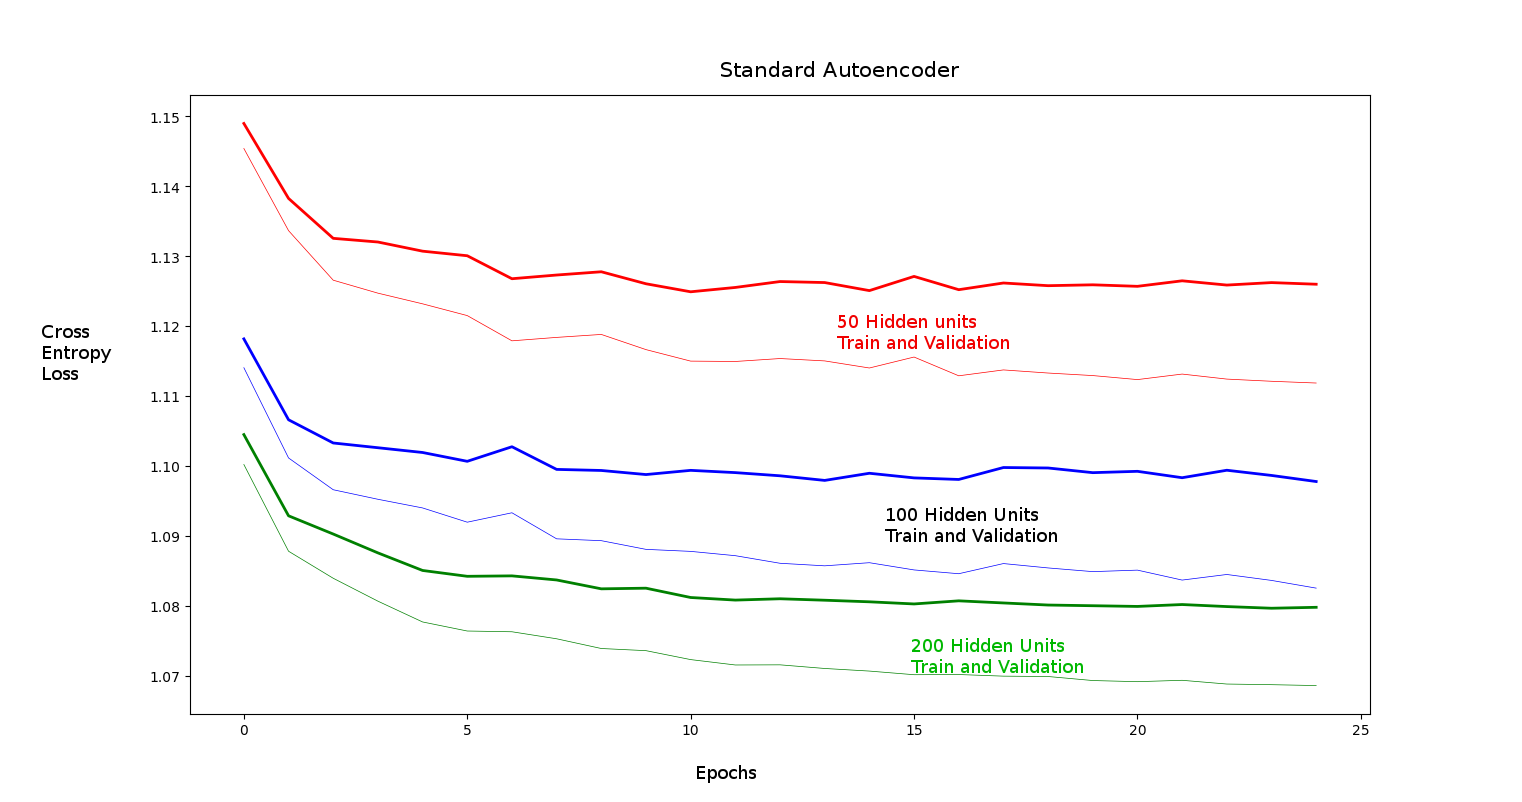
\includegraphics[scale=0.22]{ae_hu_experiment.png}
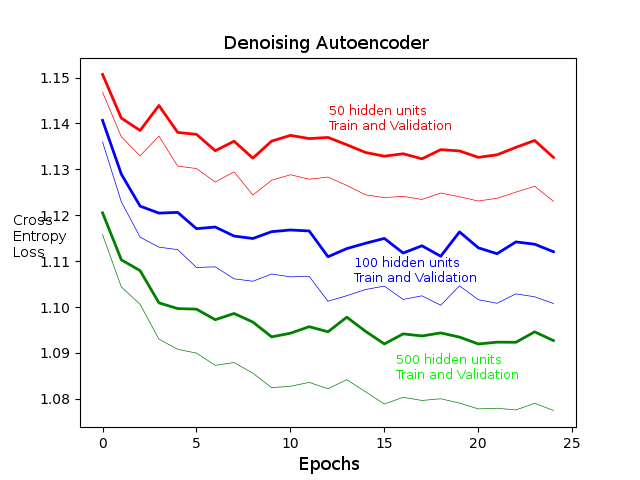
\includegraphics[scale=0.4]{ae_dropout_hu_experiment.png}

(Note: Some of the loss plots are negative log likelihood.)

The larger the hidden units, the better training and validation accuracy across all 3 settings. It follows from intuition that larger hidden units allow preserving more information about the input making the reconstruction easier. Obviously, with larger number of hidden units the gradient descent takes longer to converge given the larger number of parameters to be learnt.


\end{document}
\grid
